% routing.tex
% Kapitel 5: Auswertung

\chapter{Auswertung}
\label{chapter:auswertung}

\section{Eingesetze Technik}
\label{chapter:auswertung:technik}

Leider verfügt die in OMNeT++ enthaltene Software nicht über die Möglichkeiten, aufgezeichnete Daten in hinreichender Tiefe oder großer Menge effizient auszuwerten und erzeugt zudem regelmäßig Abstürze und falsche Ergebnisse. Somit musste ein anderer Weg gewählt werden: Die von OMNet++ erzeugten Messdaten wurden mittels \textit{scavetool}, das zum Lieferumfang gehört, nach \textit{CSV} exportiert. Nach einer weiteren Aufbereitung der Daten durch \textit{PERL}, wie dem Entfernen von nicht benötigten Dezimalstellen und der Reduzierung der Datenmenge durch einen Dropout, wurden diese mittels \textit{GnuPlot} visualisiert. Zwecks besserer Lesbarkeit wird in diesem Kapitel der Punkt als Dezimaltrennzeichen verwendet.

\begin{figure}
  \centering
  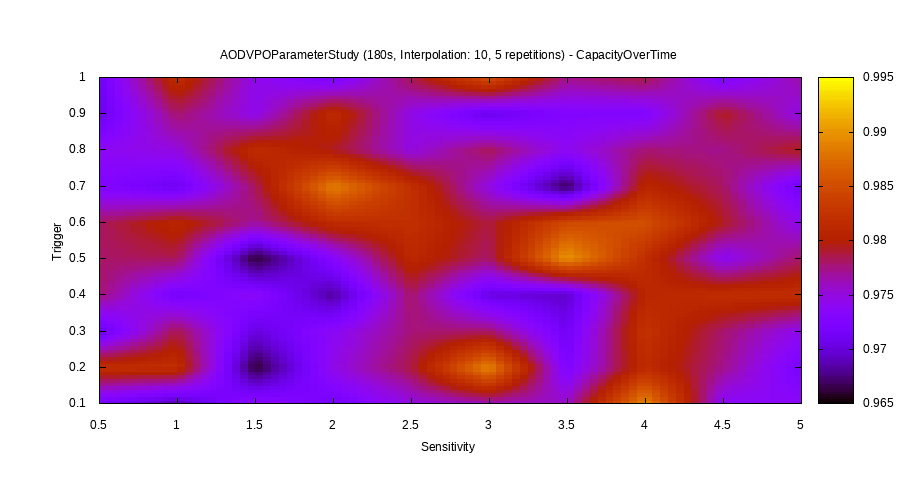
\includegraphics[scale=0.45]{bilder/aps1.png} \\
  \caption{ParameterStudy AODV nach 180 Sekunden, Abweichung der Kapazität}
  \label{image:omnet:aodv:one}
\end{figure}

\section{Die Auswertung}
\label{chapter:auswertung:versuche}

\subsection{Parameter Study}
\label{chapter:auswertung:study}

Wie zuvor beschrieben, gibt es bei beiden Protokollen die Möglichkeit die Stärke und Frequenz der Anpassung der Routingeigenschaften über Parameter zu steuern, namentlich Trigger $t$ und Sensitivität $s$. Um hierfür geeignete Werte zu ermitteln, wurde eine \textit{ParameterStudy} entworfen, die mögliche Kombinationen beider Werte in 5\% Schritten des gültigen Intervalls in mehrfacher Wiederholung testet. Die Werte dazwischen wurden interpoliert. Grundsätzlich sehen Diagramme in 3D natürlich besser aus, dennoch sind sie für eine fundierte Analyse weniger hilfreich als \textit{Heatmaps}. Daher werden im weiteren Verlauf nur Letztere gezeigt. Für alle im Rahmen der ParameterStudy gezeigten Diagramme gilt: Je höher der Wert, desto besser das Ergebnis.


\begin{figure}
  \centering
  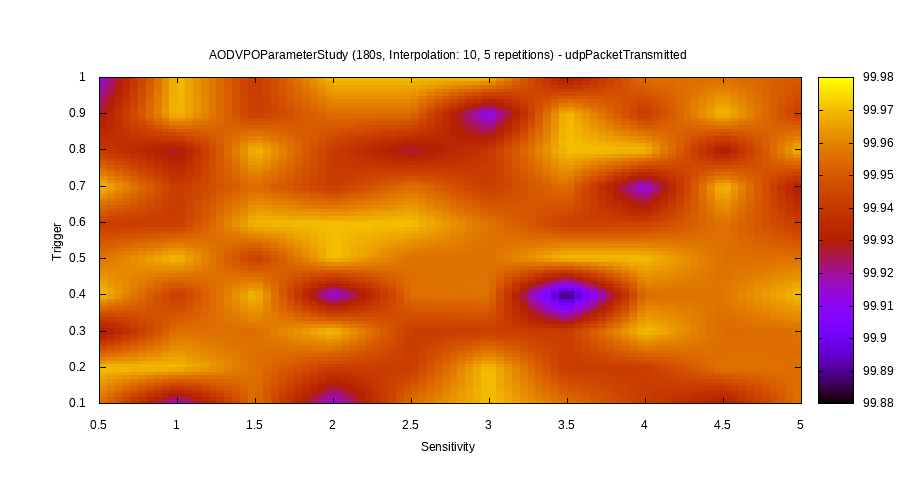
\includegraphics[scale=0.45]{bilder/aps2.png} \\
  \caption{ParameterStudy AODV nach 180 Sekunden, PacketLoss}
  \label{image:omnet:aodv:two}
\end{figure}

\subsubsection{Parameter Study - AODV}
\label{chapter:auswertung:studyaodv}

\begin{figure}
  \centering
  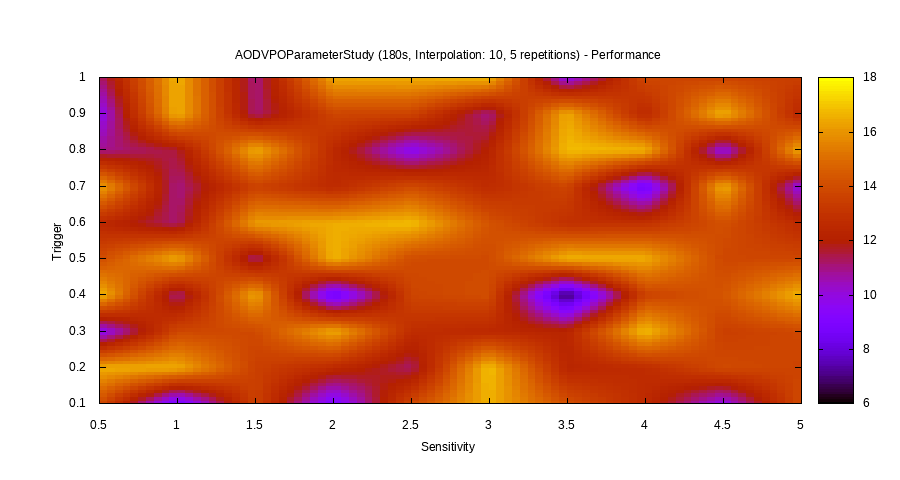
\includegraphics[scale=0.45]{bilder/aps3.png} \\
  \caption{ParameterStudy AODV nach 180 Sekunden, Performance}
  \label{image:omnet:aodv:three}
\end{figure}

In Abbildung \ref{image:omnet:aodv:one} wird die Beziehung $1-D(s,t)$ visualisiert, wobei $D$ die \textit{Standardabweichung der Kapazität} zum Ende der Simulation darstellt. Je heller der Wert, desto ähnlicher waren die Ladestände der Router. Es muss jedoch auch die Verlustrate betrachtet werden, denn was nützt ein ausgeglichener Verbrauch, wenn keine Daten mehr transportiert werden. Die Auswertung des \textit{PacketLoss} $L$ kann der Abbildung \ref{image:omnet:aodv:two} entnommen werden, wobei hier wieder $1-L(s,t)$ dargestellt wird. Wenn man beide Tests miteinander in Form der \og \textit{Performance} kombiniert, dann ergibt sich daraus Abbildung \ref{image:omnet:aodv:three}. Aus den vorliegenden Daten können nun mehrere Parameterkombinationen ermittelt werden, die zu guten Ergebnissen führen müssten, also durch eine hohe Performance sowohl einen ausgeglichenen Ladezustand herstellen, als auch mit einem geringen PacketLoss auskommen. Für die weiteren Untersuchungen wurde das Tupel $(s,t) = (4,0.3)$ gewählt. Die Auswertung des \textit{Overhead} durch das Protokoll in Abbildung \ref{image:omnet:aodv:six} zeigt, dass auch hier sehr gute Werte, die gewählte Kombination gehört zum besten Drittel, erreicht werden. Daher wurden die genannten Werte für fast alle weiteren Simulationen genutzt. Es liegen auch viele optimale Kombinationen in den Randbereichen, bei deren Verwendung kam es jedoch bei einigen Iterationen immer wieder zu ungewöhnlichen Abweichungen, die vermutlich auf ungünstige Zufallswerte zurückzuführen sind.

\begin{figure}
  \centering
  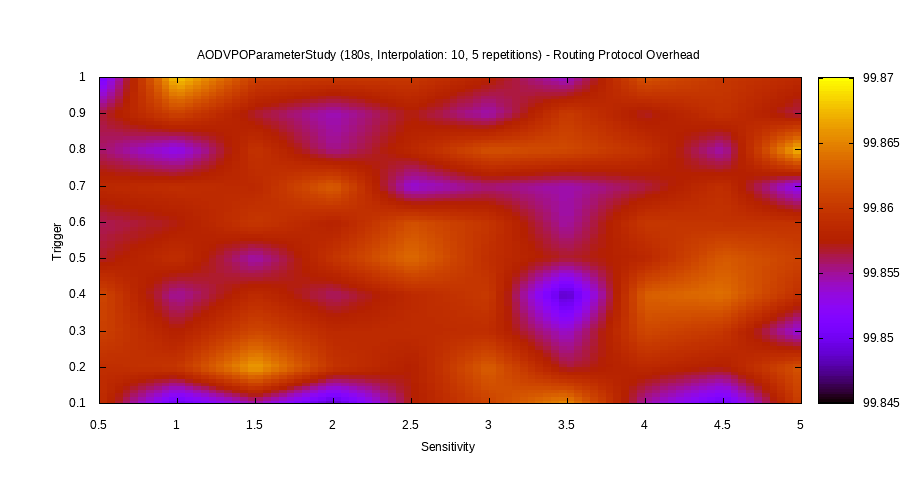
\includegraphics[scale=0.45]{bilder/aps6.png} \\
  \caption{ParameterStudy AODV nach 180 Sekunden, Routing Overhead}
  \label{image:omnet:aodv:six}
\end{figure}

\subsubsection{Parameter Study - OLSR}
\label{chapter:auswertung:studyaodv}

Hier wurden die selben Untersuchungen durchgeführt. Die Ergebnisse sind den Abbildungen \ref{image:omnet:olsr:one}, \ref{image:omnet:olsr:two}, \ref{image:omnet:olsr:three} und \ref{image:omnet:olsr:six} zu entnehmen. Es gelten die selben Aussagen wie bei \gls{aodv}. Während jedoch bei \gls{aodv} die Abweichung bis zum sechsfachen zwischen dem besten und schlechtesten Ergebnis beträgt, ist diese bei \gls{olsr} deutlich geringer, wie sich den Abbildungen entnehmen lässt. Es wurde das Tupel $(s,t) = (0{.}375 ,0{.}3)$ gewählt, da es akzeptable Ergebnisse liefert.

\begin{figure}
  \centering
  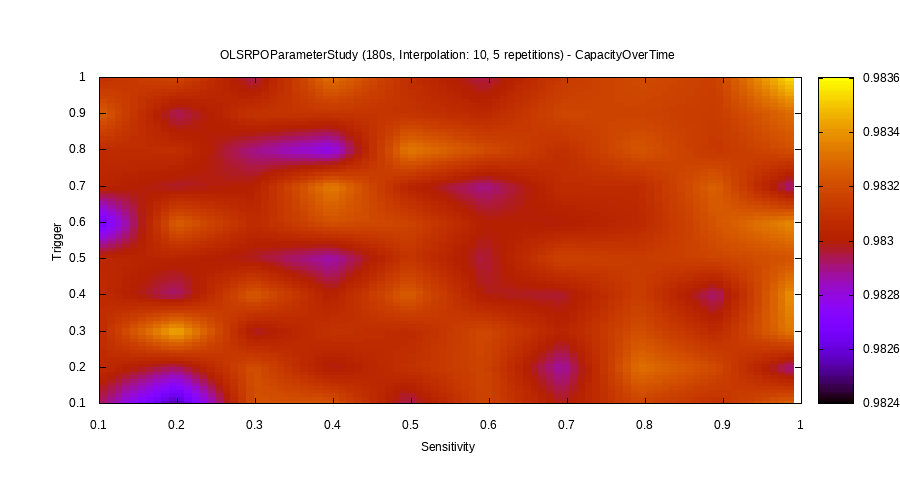
\includegraphics[scale=0.45]{bilder/ops1.png} \\
  \caption{ParameterStudy OLSR nach 180 Sekunden, Abweichung der Kapazität}
  \label{image:omnet:olsr:one}
\end{figure}

\begin{figure}
  \centering
  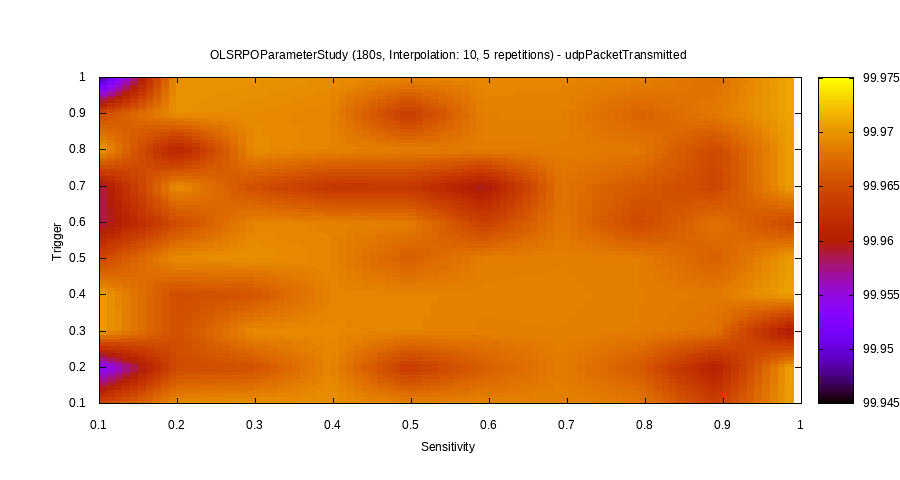
\includegraphics[scale=0.45]{bilder/ops2.png} \\
  \caption{ParameterStudy OLSR nach 180 Sekunden, PacketLoss}
  \label{image:omnet:olsr:two}
\end{figure}

\begin{figure}
  \centering
  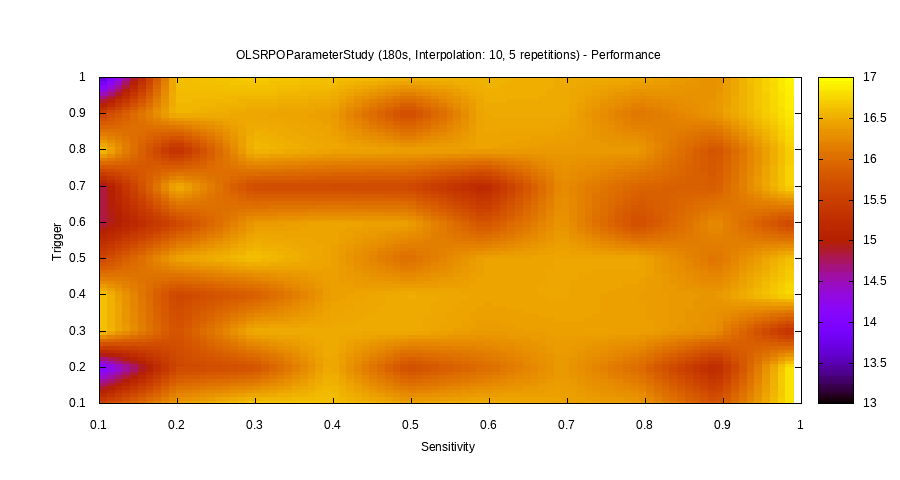
\includegraphics[scale=0.45]{bilder/ops3.png} \\
  \caption{ParameterStudy OLSR nach 180 Sekunden, Performance}
  \label{image:omnet:olsr:three}
\end{figure}

\begin{figure}
  \centering
  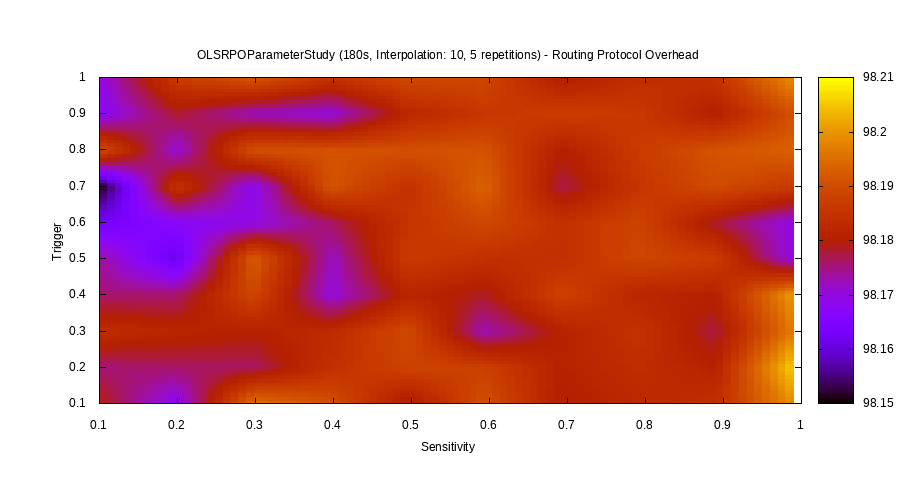
\includegraphics[scale=0.45]{bilder/ops6.png} \\
  \caption{ParameterStudy OLSR nach 180 Sekunden, Routing Overhead}
  \label{image:omnet:olsr:six}
\end{figure}

\subsection{Auswertung AODV-PO}
\label{chapter:auswertung:versuche-aodv}

Zum Vergleich der Optimierung wurde zuerst ein Single-Hop Netz (\vgl Abbildung \ref{image:omnet:aodv1}) getestet, das ausschließlich aus normalen AODV-Routern besteht. Alle Versuche wurden 100 mal mit verschiedenen Zufallszahlen wiederholt. Die Ladung der Energieversorgungen im Verlauf der Zeit ist in Abbildung   \ref{image:omnet:olsr:av1} dargestellt. Wie man sieht, wird hier immer die komplette Energie eines Routers verbraucht. Anschließend schaltet der Router ab und der nächste Router wird genutzt. Nach der Anpassung stellt sich der Energieverbrauch wie in Abbildung \ref{image:omnet:olsr:av5} dar: Nachdem eine gewisse Menge Energie verbraucht wurde, wird ein \gls{rerr} ausgelöst. Anschließend wird ein anderer Router genutzt, da er als günstigerer Pfad erkannt wird. So wird nach und nach immer wieder der Router gewechselt und der Energieverbrauch gleichmäßig verteilt.\newline

\begin{figure}
  \centering
  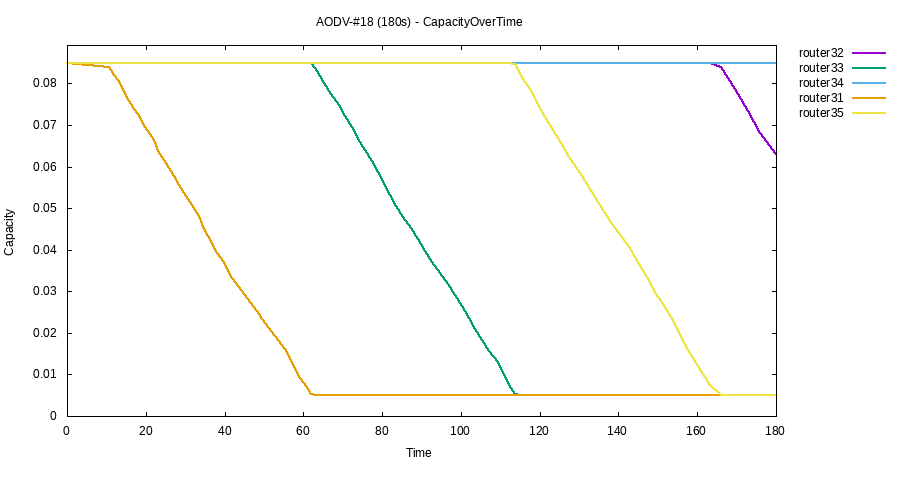
\includegraphics[scale=0.45]{bilder/av1.png} \\
  \caption{Verlauf Ladezustand bei AODV, 180 Sekunden}
  \label{image:omnet:olsr:av1}
\end{figure}

\begin{figure}
  \centering
  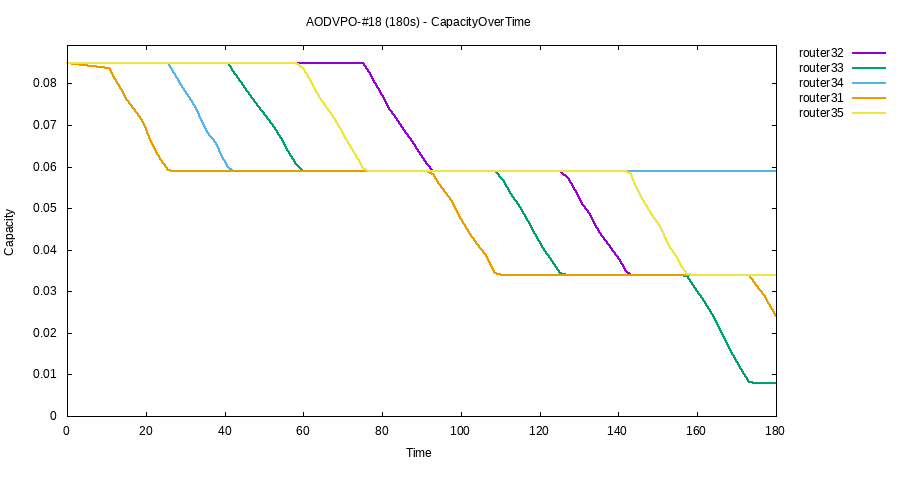
\includegraphics[scale=0.45]{bilder/av5.png} \\
  \caption{Verlauf Ladezustand bei AODV-PO, 180 Sekunden}
  \label{image:omnet:olsr:av5}
\end{figure}

Um die Wirkung eines geänderten Triggers $t$ zu testen, wurden zwei Versuche mit $t = 0.2$ (schnellere Reaktion) und $t=0.4$ (langsamere Reaktion) durchgeführt. Wie man in den Abbildungen \ref{image:omnet:olsr:av9} und \ref{image:omnet:olsr:av10} erkennen kann, werden hier die Router öfter \bzw seltener gewechselt.\newline

\begin{figure}
  \centering
  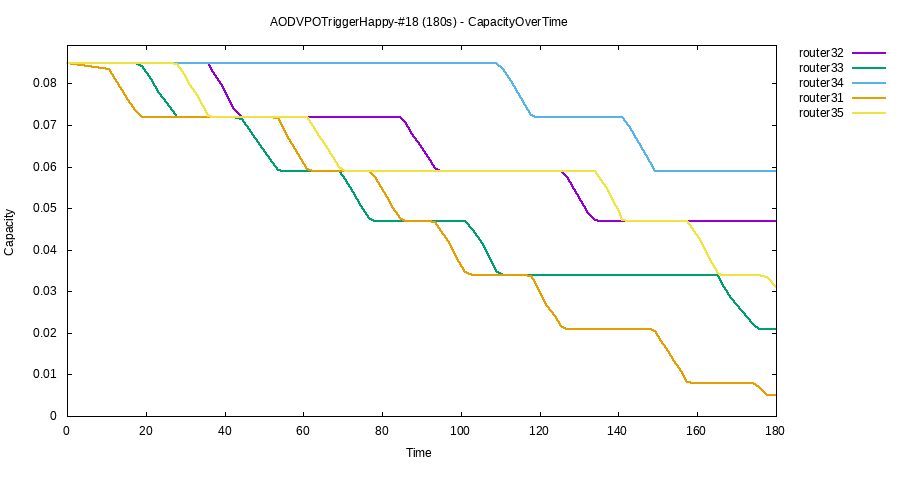
\includegraphics[scale=0.45]{bilder/av9.png} \\
  \caption{Niedrigerer Trigger $t=0.2$ bei AODV-PO, 180 Sekunden}
  \label{image:omnet:olsr:av9}
\end{figure}

\begin{figure}
  \centering
  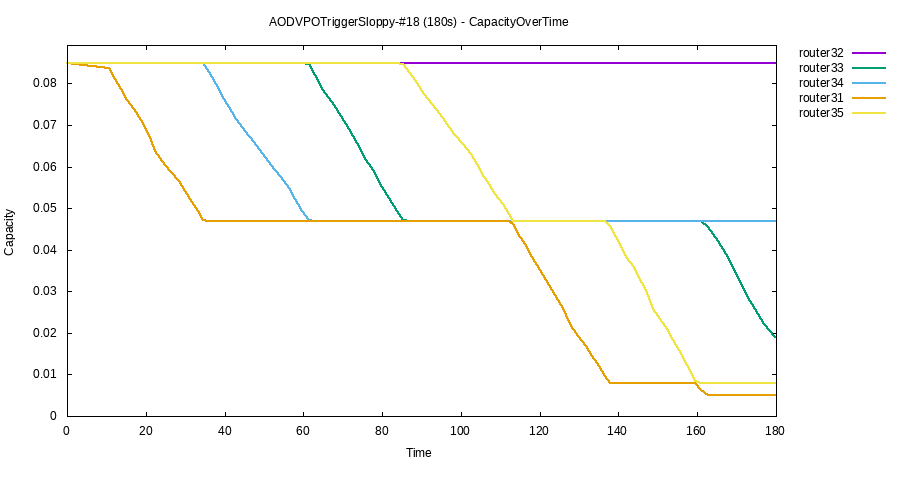
\includegraphics[scale=0.45]{bilder/av10.png} \\
  \caption{Höherer Trigger $t=0.4$ bei AODV-PO, 180 Sekunden}
  \label{image:omnet:olsr:av10}
\end{figure}

Zur Prüfung der Kompatibilität zwischen beiden Varianten des Protokolls wurde eine weitere Simulation durchgeführt. In dem Netz aus Abbildung \ref{image:omnet:olsr:netmixed} arbeiten die Router 22,23,24,42,43,44 mit normalem \gls{aodv}, die anderen mit der angepassten Version. Es funktioniert grundsätzlich, jedoch wird der Verkehr nicht so gleichmäßig wie bei den anderen Untersuchungen verteilt (\vgl Abbildung \ref{image:omnet:olsr:av11}). Auch ein Start mit unterschiedlichen Ladezuständen ist möglich. Der Verkehr wird so verteilt, dass sich diese angleichen.\newline

\begin{figure}
  \centering
  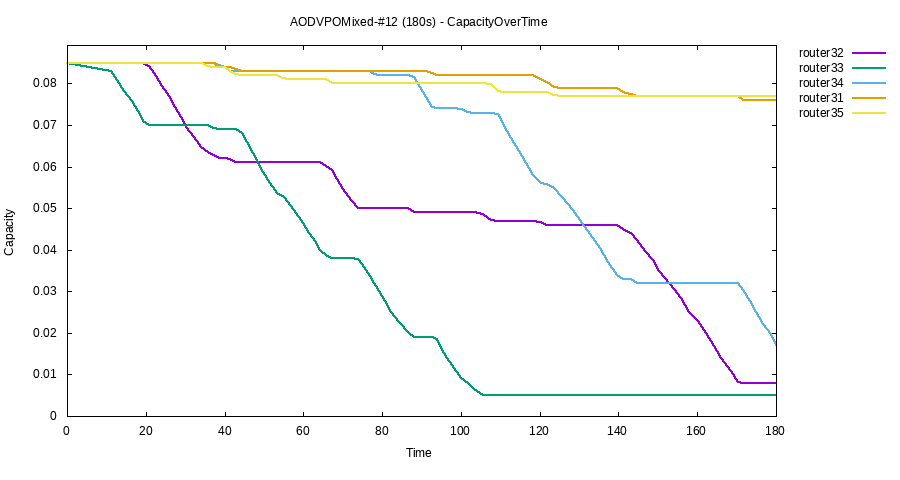
\includegraphics[scale=0.45]{bilder/av11.png} \\
  \caption{AODV und AODV-PO im Mischbetrieb, 180 Sekunden}
  \label{image:omnet:olsr:av11}
\end{figure}

\begin{figure}
  \centering
  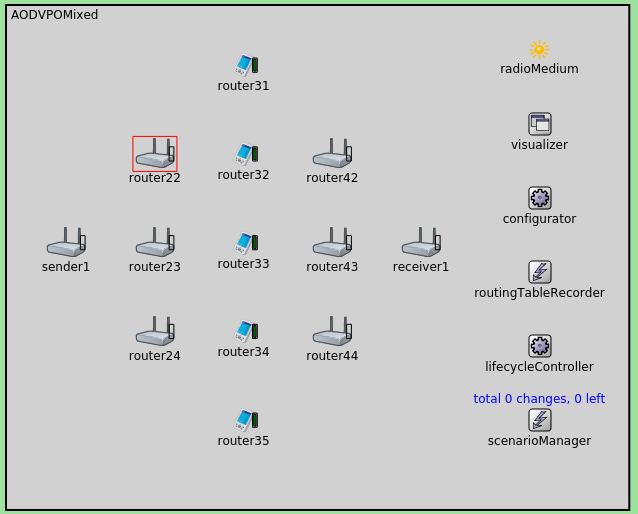
\includegraphics[scale=0.35]{bilder/netmixed.png} \\
  \caption{Netzwerk für den Mischbetrieb}
  \label{image:omnet:olsr:netmixed}
\end{figure}

Das Ziel, den Verkehr nach dem Energievorrat zu verteilen, kann als erreicht angesehen werden. Die erwünschte Kompatibilität zwischen neuem und altem Verfahren ist ebenfalls gegeben.

\subsection{Auswertung OLSR-PO}
\label{chapter:auswertung:versuche-olsr}

Für den Test der Anpassung bei \gls{olsr} wurden die selben Simulationen unter den selben Bedingungen durchgeführt. Die Ergebnisse zeigen das gleiche Verhalten wie bei \gls{aodv}. Die grafischen Auswertungen sind hier zu Gunsten der Übersichtlichkeit nicht dargestellt, sondern dem Anhang \ref{appendix:olsr} zu entnehmen. Das angestrebte Verhalten ist hier ebenfalls erreicht worden.

\subsection{Vergleich Protokolle}
\label{chapter:auswertung:vergleich}

Während die Abweichung der Ladezustände bei beiden Protokollen in der Standardversion vergleichbar hoch ist (Abbildung \ref{image:omnet:olsr:comp1}), erkennt man wie diese bei den angepassten Varianten im Durchschnitt stark abnimmt, bei \gls{olsr} sogar deutlicher. Bemerkenswert ist auch, dass die trägere Version besser als die normale ist, was jedoch mit der Laufzeit erklärbar ist (durch Zufall haben alle Ladezustände den selben Wert). Bei kürzerer oder längerer Laufzeit ergeben sich andere Werte. Der stärkere Grad der Verteilung bei dem proaktiven Verfahren fordert allerdings höheren Overhead (Abbildung \ref{image:omnet:olsr:comp2}).\newline

\begin{sidewaysfigure}
  \centering
  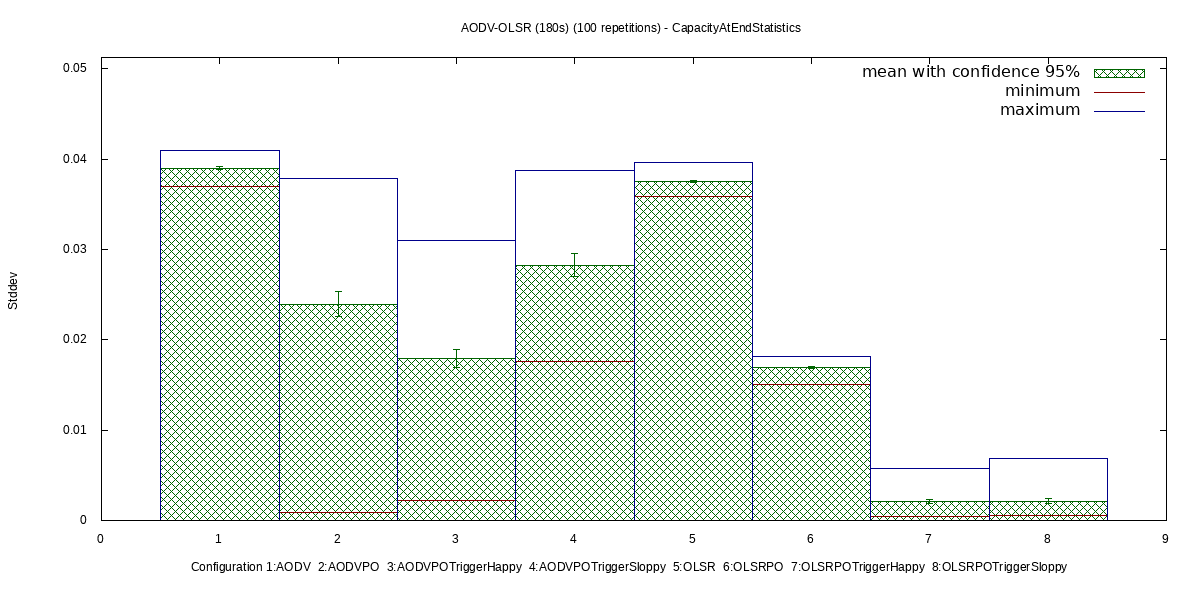
\includegraphics[scale=0.5]{bilder/c1.png} \\
  \caption{Vergleich Verlauf Ladezustand bei OLSR und AODV, 180 Sekunden}
  \label{image:omnet:olsr:comp1}
\end{sidewaysfigure}


\begin{sidewaysfigure}
  \centering
  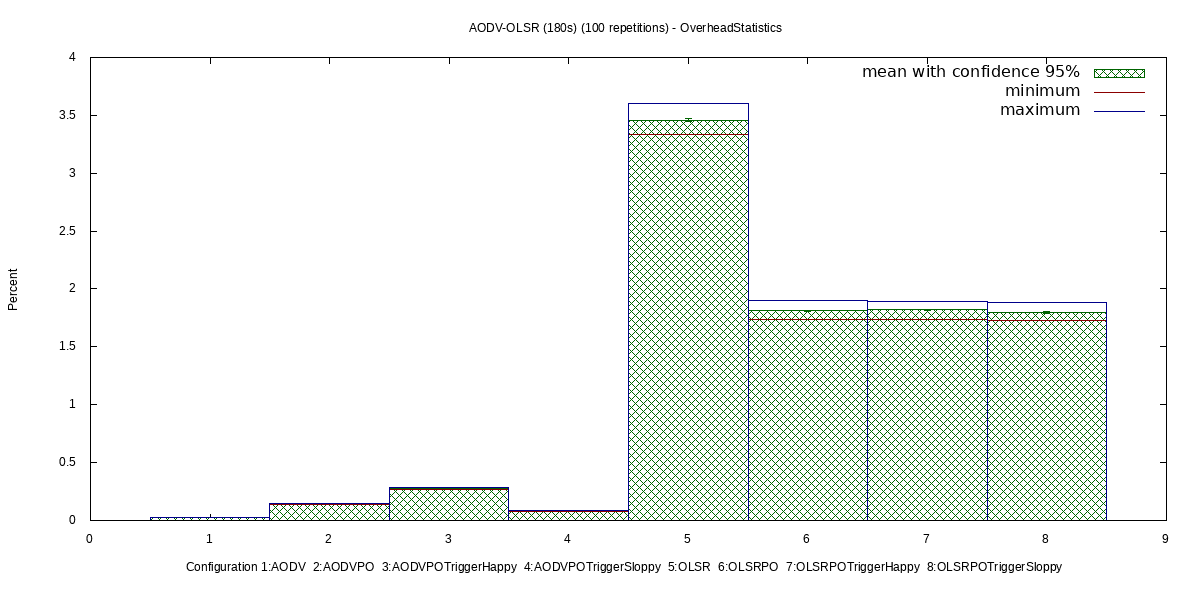
\includegraphics[scale=0.5]{bilder/c2.png} \\
  \caption{Vergleich Overhead bei OLSR und AODV, 180 Sekunden}
  \label{image:omnet:olsr:comp2}
\end{sidewaysfigure}

Der Paketverlust liegt bei den angepassten Varianten deutlich niedriger. Hier liegt \gls{olsr} zudem erheblich vor \gls{aodv}, was durch den nahtlosen Wechsel erklärt werden kann (\vgl Abbildung \ref{image:omnet:olsr:sa3} und \ref{image:omnet:olsr:so3}). Der Ausreißer bei unangepasstem OLSR ist darauf zurückzuführen, dass die Router unkontrolliert abschalten, wodurch es erst eine Weile dauert, bis wieder neue Routen gewählt werden und in der Zwischenzeit Pakete verloren gehen.

\begin{figure}
  \centering
  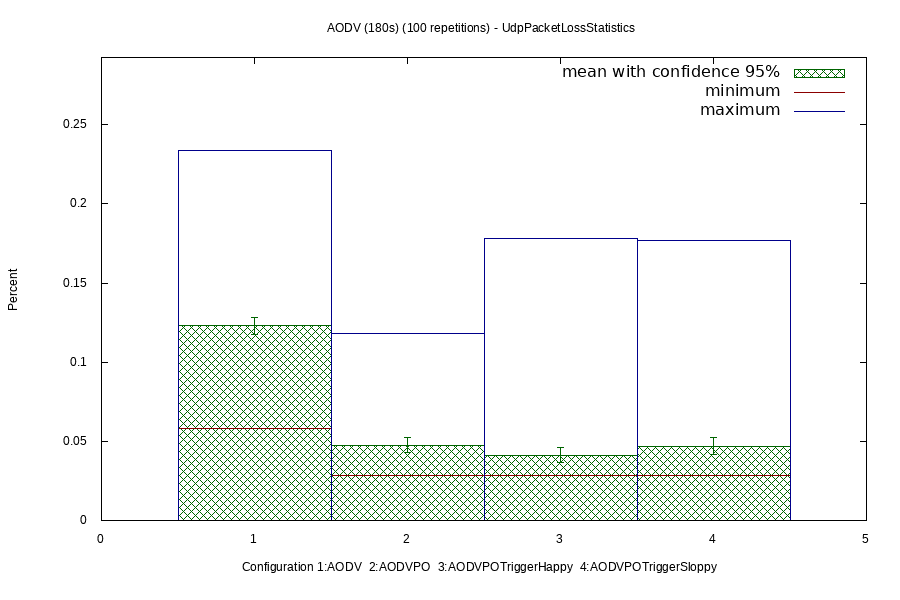
\includegraphics[scale=0.4]{bilder/sa3.png} \\
  \caption{Vergleich PacketLoss bei AODV, 180 Sekunden}
  \label{image:omnet:olsr:sa3}
\end{figure}

\begin{figure}
  \centering
  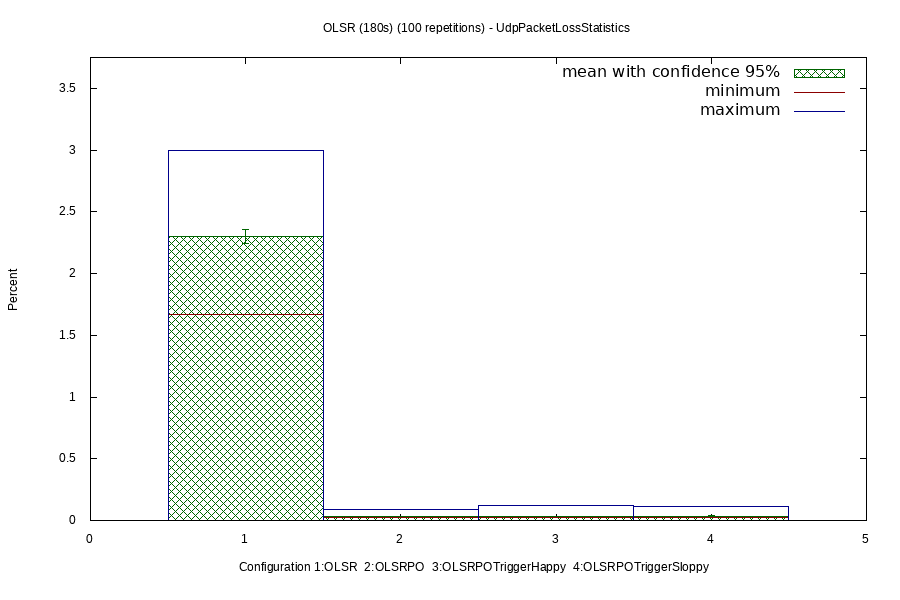
\includegraphics[scale=0.4]{bilder/so3.png} \\
  \caption{Vergleich PacketLoss bei OLSR, 180 Sekunden}
  \label{image:omnet:olsr:so3}
\end{figure}

\subsection{Weitere Erkenntnisse}
\label{chapter:auswertung:erkenntnisse}

Die Simulation wurden mit hundert Wiederholungen durchgeführt. Es zeigt sich, dass die Anpassungen beider Protokolle stabil Ihre Wirkung entfalten. Auch hierzu sind im Anhang \ref{appendix:repeat} entsprechende Auswertungen beigefügt. Es fällt auf, dass die Ergebnisse bei \textit{OLSR-PO} stärker streuen, dennoch sind diese konstant niedriger als bei \gls{olsr}. Darüber hinaus wurde das Verhalten in einem größeren Netz (Abbildung \ref{image:omnet:aodv2}) überprüft. Die Funktion ist dort ebenfalls gegeben, auch wenn es zu stärkeren Abweichungen kommt. \textit{AODV-PO} verhält sich zum Ende der Simulation instabil, die Ursache hierfür konnte nicht abschließend geklärt werden. Hierzu sind entsprechende Auswertungen im Anhang \ref{appendix:multihop} zu finden. Bei der letzten Untersuchung galt es, den Vorteil von proaktiven Protokollen bei vielen verschiedenen Zielen zu untersuchen. Hierzu wurden die Pakete zufällig auf alle Hosts im MultiHop-Netz verteilt. Hier zeigt OLSR ein leicht geringere Verlustrate von Paketen, da die Routen sofort zur Verfügung stehen und nicht erst ermittelt werden müssen, was zu Zeitüberschreitungen und damit zum Verwerfen der Pakete führt (Abbildung \ref{image:omnet:olsr:comp3}). Es ist anzunehmen, dass dieser Vorteil mit wachsender Größe des Netzes zunehmen wird.

\begin{sidewaysfigure}
  \centering
  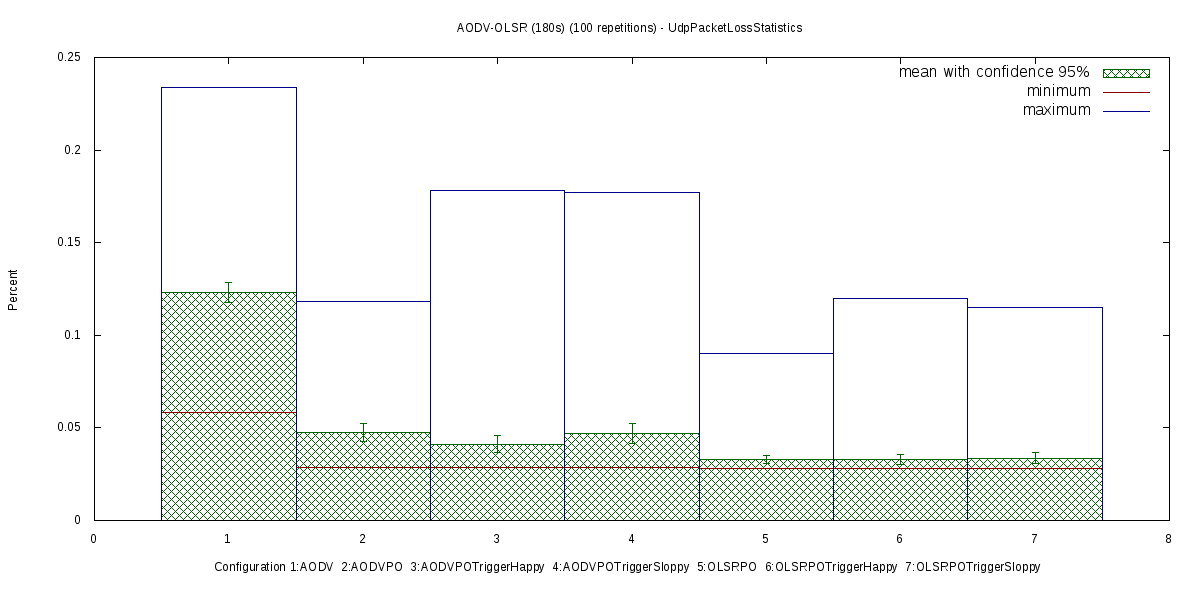
\includegraphics[scale=0.5]{bilder/c3.png} \\
  \caption{Vergleich Verlustrate Multi-Recipient bei OLSR und AODV, 180 Sekunden}
  \label{image:omnet:olsr:comp3}
\end{sidewaysfigure}